
% Maybe some stuff about template metaprogramming in this chapter?

\chapter{User documentation}

\section{Target audience}

This document expects the reader to have a basic understanding of template
metaprogramming in C++.

%TODO

\section{Main concepts}

Mihalicza relates concepts in traditional run time programs and C++ template
metaprograms\cite{mihalicza-phd}:

\begin{center}
    \begin{tabular}{| c | c |}
        \hline
        Run time execution & C++ TMP execution \\ \hline \hline
        function call & template instantiation \\ \hline
        call stack & instantiation stack \\ \hline
        function parameter & template parameter \\ \hline
        return value & the referenced nested type \\ \hline
        function body & template definition \\
        \hline
    \end{tabular}
\end{center}

He also compares debug operations between run time and metaprograms:

\begin{center}
    \begin{tabular}{| c | c |}
        \hline
        Run time debug operation & C++ TMP debug operation \\ \hline \hline
        step in/over/out functon call & step in/over/out instantiation \\ \hline
        continue execution & continue compilation \\
        \hline
    \end{tabular}
\end{center}


%TODO

\section{Installation}

Metashell supports the following platforms:
\begin{itemize}
    \item Linux
    \item FreeBSD
    \item OpenBSD
    \item OS X
    \item Windows
\end{itemize}

In this section, installation instructions only for Linux is described.
Instructions for other platforms can be found in the README.md file shipped
with Metashell.

\subsection{Dependencies}

Install the dependent libraries and tools:

\begin{itemize}
    \item Termcap and Readline (version 6.3 or newer)
    \item CMake (2.18.12.2 or newer)
\end{itemize}

Acquire the source code from Github\cite{github} or any release site, and cd
into the source directory:

\begin{itemize}
    \item \texttt{cd metashell}
\end{itemize}

Build Clang with Templight\cite{templight}:

\begin{itemize}
    \item \texttt{cd templight}
    \item \texttt{mkdir build}
    \item \texttt{cd build}
    \item \texttt{cmake ../llvm -DLIBCLANG\_BUILD\_STATIC=ON}
    \item \texttt{make clang}
    \item \texttt{make libclang}
    \item \texttt{make libclang\_static}
    \item \texttt{cd ..}
\end{itemize}

\subsection{Building}

Now compile Metashell:

\begin{itemize}
    \item \texttt{mkdir bin}
    \item \texttt{cd bin}
    \item \texttt{cmake ..}
    \item \texttt{make}
\end{itemize}

The most important files that got compiled in this step (paths are relative to
the bin directory):

\begin{description}
    \item[\texttt{app/metashell}:] The program executable
    \item[\texttt{test/metashell\_test}:] Test executable
\end{description}

\subsection{Running tests}

To make sure everything will work correctly, running tests is advised:

\begin{itemize}
    \item \texttt{test/metashell\_test}
\end{itemize}

\section{Basic Usage\cite{github}} %TODO cite this whole thing?

\subsection{Starting metadebugger}

Start metashell by running \texttt{app/metashell}.

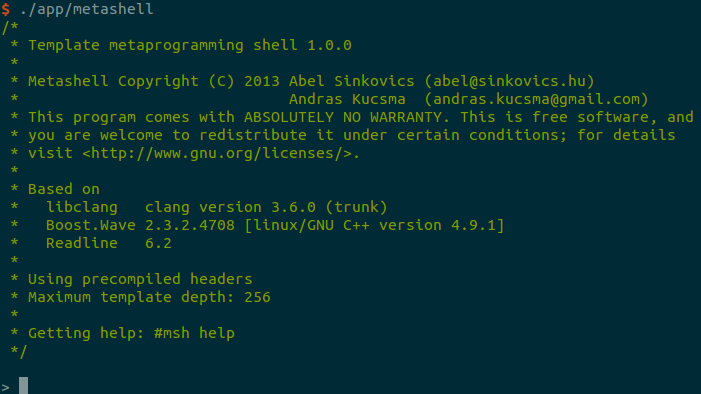
\includegraphics[width=0.9\textwidth]{img/splash.eps}

%TODO maybe mention, that "> " is metashell?
After a splash screen is shown, an interactive shell with \texttt{"> "}
prompt string appears. This is the place, where the C++ code environment
required by the metaprogram can be entered.

As an example, let's enter the fibonacci metaprogram mentioned earlier:

\lstset{
    numbers=none
}
\begin{lstlisting}[escapechar=, style=mdboutput]
> template<int N> struct fib { \
...>static const int value = \
...>   fib<N - 1>::value + \
...>   fib<N - 2>::value; \
...>};
> template<> struct fib<1> { static const int value = 1; };
> template<> struct fib<0> { static const int value = 0; };
> template<int N> struct int_ {};
\end{lstlisting}

By entering backslashes at the end of the lines, you can enter longer lines
easily.

Now start the metadebugger by entering:

\begin{lstlisting}[escapechar=, style=mdboutput]
> #msh mdb int_<fib<6>::value>
For help, type "help".
Metaprogram started
\end{lstlisting}

You'll see, that the prompt has changed to \texttt{"(mdb) "}. Now you can enter
metadebugger commands.

\subsection{Stepping}

Metadebugger provides an interface similar to gdb. For example you can step the
metaprogram forward three steps:

\begin{lstlisting}[escapechar=, style=mdboutput]
(mdb) step 3
fib<4> (TemplateInstantiation)
\end{lstlisting}

As you can see, metadebugger tells you that in this step \texttt{fib<4>} is
getting instantiated in a \texttt{TemplateInstantiation} event.

Stepping backwards is also trivial in a template metaprogram:

\begin{lstlisting}[escapechar=, style=mdboutput]
(mdb) step -1
fib<5> (TemplateInstantiation)
\end{lstlisting}

\subsection{Backtrace}

You can check the current backtrace:

\begin{lstlisting}[escapechar=, style=mdboutput]
(mdb) bt
#0 fib<5> (TemplateInstantiation)
#1 fib<6> (TemplateInstantiation)
#2 int_<fib<6>::value>
\end{lstlisting}

This shows us that:

\begin{itemize}
    \item
        We started the template metaprogram execution by evaluating
        \texttt{int\_<fib<6>::value>}.
    \item
        The evaluation of this expression has (at some point) called
        \texttt{fib<6>}.
    \item
        The fib metafunction has (at some point) called \texttt{fib<5>}.
        This is where we are in the execution of the metaprogram.
\end{itemize}

\subsection{Forwardtrace}

Metadebugger can also see into the future, and print the forwardtrace from any
step:

\begin{lstlisting}[escapechar=, style=mdboutput]
(mdb) ft
fib<5> (TemplateInstantiation)
+ fib<4> (TemplateInstantiation)
| + fib<3> (TemplateInstantiation)
| | + fib<2> (TemplateInstantiation)
| | | + fib<1> (Memoization)
| | | ` fib<0> (Memoization)
| | ` fib<1> (Memoization)
| ` fib<2> (Memoization)
` fib<3> (Memoization)
\end{lstlisting}

This shows us what metafunctions the metaprogram \textit{will} call after the
current location. As you can see the output shows the relations between the
function calls: which metafunction calls which other metafunctions. The events
in the output of forwardtrace happen in that order from the top down.

You probably noticed that there are two kinds of events metadebugger shows you:

\begin{description}
    \item[TemplateInstantiation] event happens when the compiler first
        encounters and instantiates a new template type. During a
        \texttt{TemplateInstantiation} event the compiler will instantiate
        every subtype it needs to get to the result
    \item[Memoization] event happens when a compiler encounters a type, which
        it had already instantiated before. It won't go through the
        instantiation process again, instead it uses technique called
        memoization to speed up the compilation. This basically means that the
        compiler remembers every type it had instantiated, and reuses them when
        it encounters them again.

        Full template specializations (e.g. \texttt{fib<0>} and
        \texttt{fib<1>}) only appear in Memoization events.
\end{description}

For example, in the above forwardtrace output, you can see that \texttt{fib<5>}
reates \texttt{fib<4>} in a \texttt{TemplateInstantiation} event, which in turn
instantiates \texttt{fib<3>} also in a \texttt{TemplateInstantiation} event and
so on.  You can also see, that when \texttt{fib<5>} gets to the point to
instantiate \texttt{fib<3>} it has already been instantiated by
\texttt{fib<4>}, so only a \texttt{Memoization} event happens.

\subsection{Breakpoints and continue}

You can also create breakpoints:

\begin{lstlisting}[escapechar=, style=mdboutput]
(mdb) rbreak fib<3>
Breakpoint "fib<3>" will stop the execution on 2 locations
\end{lstlisting}

Now let's continue the execution until the first breakpoint:

\begin{lstlisting}[escapechar=, style=mdboutput]
(mdb) continue
Breakpoint "fib<3>" reached
fib<3> (TemplateInstantiation)
\end{lstlisting}

Commands can be abbreviated if unambigouos. For example you can use just
\texttt{c} instead of \texttt{continue}:

\begin{lstlisting}[escapechar=, style=mdboutput]
(mdb) c
Breakpoint "fib<3>" reached
fib<3> (Memoization)
\end{lstlisting}

You can repeat the last command by simply hitting enter again:

\begin{lstlisting}[escapechar=, style=mdboutput]
(mdb)
Metaprogram finished
mpl_::int_<13>
\end{lstlisting}

\subsection{Full mode}

There are two modes which Metadebugger can operate in. The normal mode, which
was shown in the previous chapters, and the full mode. To demonstrate the
difference let's evaluate a metaprogram in full mode and print the
forwardtrace:

\begin{lstlisting}[escapechar=, style=mdboutput]
(mdb) evaluate -full int_<fib<4>::value>
Metaprogram started
(mdb) ft
int_<fib<4>::value>
+ fib<4>
| + fib<3>
| | + fib<2>
| | | + fib<1>
| | | ` fib<0>
| | ` fib<1>
| ` fib<2>
|   + fib<1>
|   ` fib<0>
` mpl_::int_<5>
\end{lstlisting}

\lstset{
    numbers=left
}

Full mode doesn't try to follow what the real complier does, but instead it
tries to simulate a dumb compiler, which doesn't use memoizations to speed up
compilation. For example, \texttt{fib<2>} and it's full sub call tree is
visible two times. This mode can be useful, when the part of the trace you're
intrested in is hidden under multiple layers of Memoizations in normal mode.

\section{Command reference}

In the following section, the following notations are used: command parameters
that are in square brackets are optional. Parameters that are between angle
brackets have to be replaced by the user with something.

\subsection{evaluate}

Usage: \verb$evaluate [-full] [<type>]$

Evaluate and start debugging a new metaprogram.

Evaluating a metaprogram using the \verb$-full$ qualifier will expand all
Memoization events.

If called without <type>, then the last evaluated metaprogram will be
reevaluated.

Previous breakpoints are cleared.

Unlike metashell, evaluate doesn't use metashell::format to avoid cluttering
the debugged metaprogram with unrelated code. If you need formatting, you can
explicitly enter \verb$metashell::format< <type> >::type$ for the same effect.

\subsection{step}

Usage: \verb$step [over] [n]$

Step the program.

Argument n means step n times. n defaults to 1 if not specified.
Negative n means step the program backwards.

Use of the \verb$over$ qualifier will jump over sub instantiations.

\subsection{rbreak}

Usage: \verb$rbreak <regex>$

Add breakpoint for all types matching \verb$<regex>$.



\subsection{continue}

Usage: \verb$continue [n]$

Continue program being debugged.

The program is continued until the nth breakpoint or the end of the program
is reached. n defaults to 1 if not specified.
Negative n means continue the program backwards.

\subsection{forwardtrace}

Usage: \verb$forwardtrace|ft [n]$

Print forwardtrace from the current point.

The n specifier limits the depth of the trace. If n is not specified, then the
trace depth is unlimited.

\subsection{backtrace}

Usage: \verb$backtrace|bt $

Print backtrace from the current point.



\subsection{help}

Usage: \verb$help [<command>]$

Show help for commands.

If <command> is not specified, show a list of all available commands.

\subsection{quit}

Usage: \verb$quit $

Quit metadebugger.





